\documentclass{beamer}
\usepackage[utf8]{inputenc}

\usetheme{Madrid}
\usecolortheme{default}
\usepackage{amsmath,amssymb,amsfonts,amsthm}
\usepackage{txfonts}
\usepackage{tkz-euclide}
\usepackage{listings}
\usepackage{adjustbox}
\usepackage{array}
\usepackage{tabularx}
\usepackage{gvv}
\usepackage{lmodern}
\usepackage{circuitikz}
\usepackage{tikz}
\usepackage{graphicx}

\setbeamertemplate{page number in head/foot}[totalframenumber]

\usepackage{tcolorbox}
\tcbuselibrary{minted,breakable,xparse,skins}



\definecolor{bg}{gray}{0.95}
\DeclareTCBListing{mintedbox}{O{}m!O{}}{%
	breakable=true,
	listing engine=minted,
	listing only,
	minted language=#2,
	minted style=default,
	minted options={%
		linenos,
		gobble=0,
		breaklines=true,
		breakafter=,,
		fontsize=\small,
		numbersep=8pt,
		#1},
	boxsep=0pt,
	left skip=0pt,
	right skip=0pt,
	left=25pt,
	right=0pt,
	top=3pt,
	bottom=3pt,
	arc=5pt,
	leftrule=0pt,
	rightrule=0pt,
	bottomrule=2pt,
	toprule=2pt,
	colback=bg,
	colframe=orange!70,
	enhanced,
	overlay={%
		\begin{tcbclipinterior}
			\fill[orange!20!white] (frame.south west) rectangle ([xshift=20pt]frame.north west);
	\end{tcbclipinterior}},
	#3,
}
\lstset{
	language=C,
	basicstyle=\ttfamily\small,
	keywordstyle=\color{blue},
	stringstyle=\color{orange},
	commentstyle=\color{green!60!black},
	numbers=left,
	numberstyle=\tiny\color{gray},
	breaklines=true,
	showstringspaces=false,
}
\begin{document}

\title 
{5.13.66}
\date{26 September,2025}

\author 
{Naman Kumar-EE25BTECH11041}
\graphicspath{./figs}


\frame{\titlepage}
\begin{frame}{Question c)}
Let p be an odd prime number and $\vec{T_p}$ be the following set of $2\times2$ matrices
\begin{align}
\vec{T_p}=\cbrak{\Vec{A}=\begin{pmatrix}a&b\\c&a\end{pmatrix}:a,b,c \in \cbrak{0,1,2,\dots,p-1} }
\end{align}
c) The number of A in $\vec{T_p}$ such that det(A) is not divisible by p is
\end{frame}
\begin{frame}{Solution}
\begin{align}
    det(\vec{A})=\begin{vmatrix}a&b\\c&a\end{vmatrix}\\
    =a^2-bc\\
\end{align}
Total number of possible matrices
\begin{align}
    =p\times p \times p=p^3
\end{align}
\end{frame}
\begin{frame}{Solution}
We can find number of matrices whose determinant is divisible by p\\
Required number = Total - number of matrices whose determinant is divisible by p
\begin{align}
    a^2-bc \equiv 0 \mod p \\
    a^2\equiv bc \mod p
\end{align}
Case 1: a=0
\begin{align}
    bc \equiv 0 \mod p
\end{align}
\end{frame}
\begin{frame}{Solution}
i) b=0, c as p-1 choices
\begin{align}
    \text{number of cases} = 1\times p=p
\end{align}
ii) c=0, b as p-1 choices
\begin{align}
    \text{number of cases} = 1\times p=p\\
    \text{total in this case}= 2(p)-1\label{1}
\end{align}
\end{frame}
\begin{frame}{Solution}
-1 for extra case of overlap at 'b' and 'c' both zero\\
Case 2: $a\neq0$\\
let $a^2=k$
\begin{align}
    \text{'a' has p-1 choices}\\
    bc \equiv k \mod p\\
    c\equiv k.b^{-1} \mod p \text{ ($b^{-1}$multiplicative inverse of b modulo p)}
\end{align}
\end{frame}
\begin{frame}{Solution}
For every 'b' we have a fixed 'c' for their are p-1 pairs of (b,c)
\begin{align}
    \text{number of cases}= (p-1)\times(p-1)=(p-1)^2 \label{2}
\end{align}
Finally adding total number cases from $\eqref{1}$ and $\eqref{2}$
\begin{align}
    =2p-1+(p^2-2p+1)
    =p^2 \label{3}
\end{align}
\end{frame}
\begin{frame}{Solution}
Finally required value is
\begin{align}
    \text{required ans}=total - \eqref{3}\\
    = p^3-p^2
\end{align}
\end{frame}
\begin{frame}{figure}
    \begin{figure}[H]
    \centering
    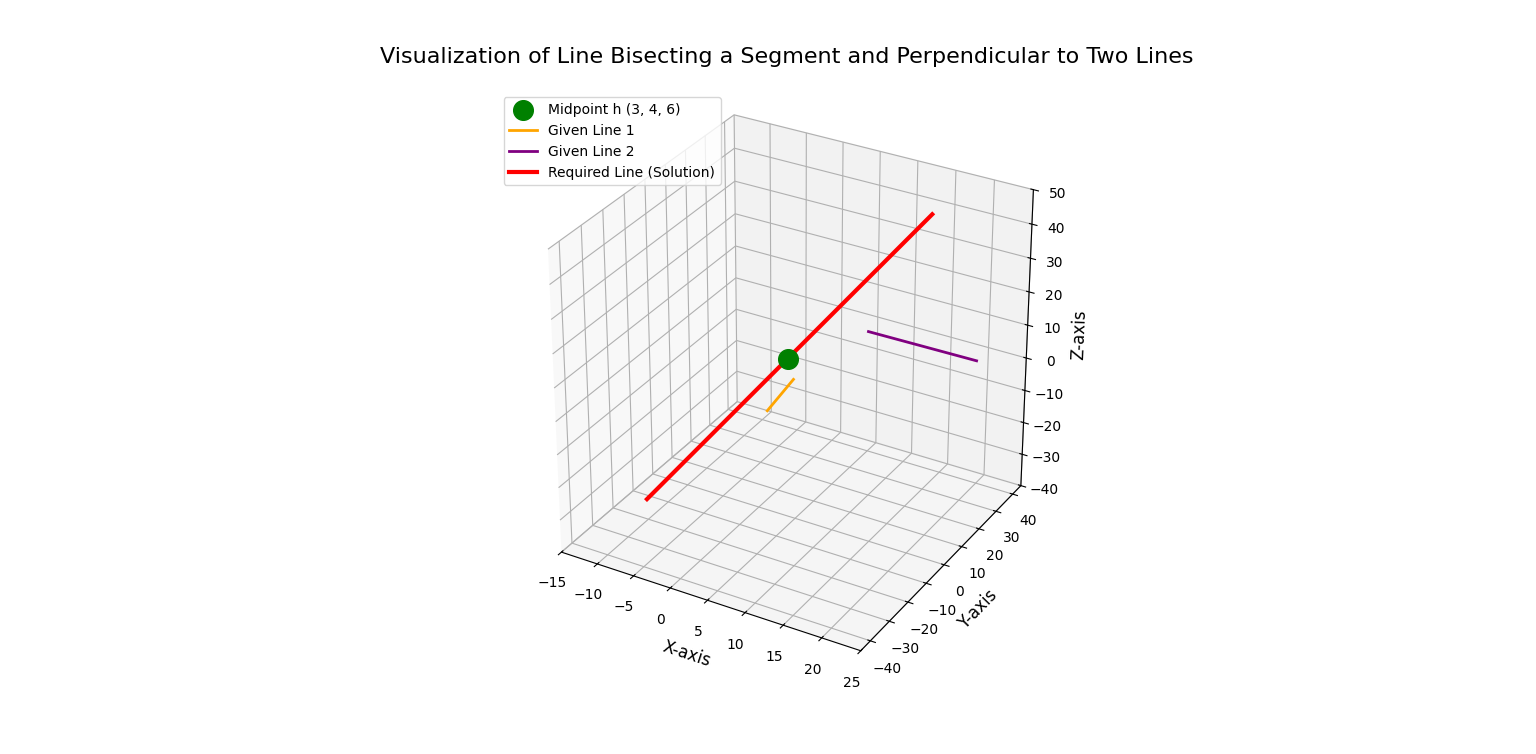
\includegraphics[width=\columnwidth]{figs/figure_c.png}
    \caption{}
    \label{fig:placeholder}
\end{figure}
\end{frame}
\end{document}